\section{Poisson Proceess}

A \underline{poisson process} is the continuous time analog of
``coin flipping'' or Bernoulli processes. This makes it a good model for
arrival processes: photons hitting a detector, packets in a network,
number of emails per hour, etc.

\begin{center}
  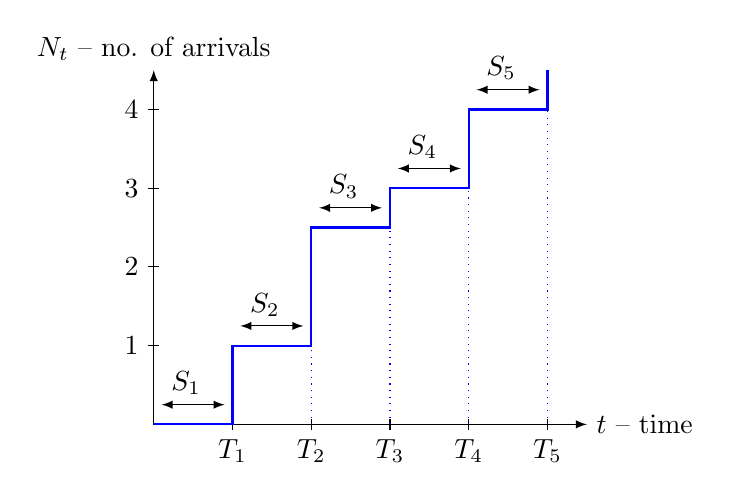
\begin{tikzpicture}[>=latex]
    \draw [<->] (0, 4.5) node [above] {$N_t$ -- no. of arrivals} |-
    (5.5, 0) node [right] {$t$ -- time};
    \foreach \x [evaluate=\x as \y using \x] in {1,...,5} \draw
    (\x,2pt) -- (\y, -2pt) node [below] {$T_{\x}$};
    \foreach \x [evaluate=\x as \y using \x] in {1,...,4} \draw
    (2pt,\x) -- (-2pt, \y) node [left] {\x};
    \draw [blue,thick] (0,0) -| (1,1) -| (2,2.5) -| (3,3) -| (4,4) -| (5,4.5);
    \draw [blue,dotted] (2,0) -- (2,1);
    \draw [blue,dotted] (3,0) -- (3,2.5);
    \draw [blue,dotted] (4,0) -- (4,3);
    \draw [blue,dotted] (5,0) -- (5,4);
    \draw [<->] (0.1,0.25) node [above right] {$S_1$} -- (0.9,0.25);
    \draw [<->] (1.1,1.25) node [above right] {$S_2$} -- (1.9,1.25);
    \draw [<->] (2.1,2.75) node [above right] {$S_3$} -- (2.9,2.75);
    \draw [<->] (3.1,3.25) node [above right] {$S_4$} -- (3.9,3.25);
    \draw [<->] (4.1,4.25) node [above right] {$S_5$} -- (4.9,4.25);
  \end{tikzpicture}
\end{center}

Each $T_i$ for $i = 1,2,3,4,5$ represents an arrival and generally,
each arrival time is defined as

\begin{displaymath}
  T_n = \sum_{i=1}^{n} S_i
\end{displaymath}

where the interarrival times
$S_1,S_2,\ldots,S_n \overset{\textrm{iid}}{\sim} Exponential(\lambda)$.
Thus, every $S_i$ has the probability density function

\begin{displaymath}
  f_{S_i}(t) = \lambda e^{\lambda t};\ t > 0;\ i=1,2,3,\ldots
\end{displaymath}

and cumulative distribution function

\begin{displaymath}
  F_{S_i}(t) = 1 - e^{-\lambda t}
  .
\end{displaymath}

\begin{definition}[Number of Arrivals]

  \begin{displaymath}
    N_t =
    \begin{cases}
      \max_{n \geq 1} \{n \mid T_n \leq t\} & t \geq 0 \\
      0 & t < T_1
    \end{cases}
  \end{displaymath}

\end{definition}

\begin{itemize}
  \item Recall: $Exponential(\lambda)$ is a memoryless RV
    \begin{enumerate}
      \item $F_{\tau}(t) =
        \begin{cases}
          1 - e^{-\lambda t} & t \geq 0 \\
          0 & t < 0
        \end{cases} \Rightarrow f_{\tau}(t) = \lambda e^{-\lambda t}$
      \item $\E\left[\tau\right] = \frac{1}{\lambda}$ and $\Var(\tau)
        = \frac{1}{\lambda^2}$
      \item $P(\tau > t + s \mid \tau > s) = P(\tau > t)$
      \item $P(\tau \leq t + \epsilon \mid \tau > t) = \lambda
        \epsilon +o(\epsilon);\ \lim_{\epsilon \rightarrow 0} \frac{o(\epsilon)}{\epsilon} = 0$
    \end{enumerate}
\end{itemize}

\begin{proof}

  \begin{align*}
    P(\tau > t + \epsilon \mid \tau > t) &= P(\tau > \epsilon) \\
                                         &= e^{-\lambda \epsilon} \\
                                         &= 1 - \lambda \epsilon + o(\epsilon)
  \end{align*}

\end{proof}

